\documentclass{article}
\usepackage{fullpage,graphicx}
\usepackage{amsmath,amsfonts,amsthm,amssymb,multirow,xcolor}
\usepackage{algorithmic}
\usepackage[ruled,vlined,commentsnumbered,titlenotnumbered]{algorithm2e}
\usepackage{minted}
\usepackage{multicol}
\usepackage{tikz}
\usetikzlibrary{positioning}


\usepackage{pgfplots}
\pgfplotsset{compat=1.10}
\usetikzlibrary{shapes.geometric,arrows,fit,matrix,positioning}
\tikzset
{
  treenode/.style = {circle, draw=black, align=center, minimum size=1cm},
  subtree/.style  = {isosceles triangle, draw=black, align=center, minimum height=0.5cm, minimum width=1cm, shape border rotate=90, anchor=north}
}

\begin{document}
\noindent
CS 161 \hfill \textbf{Homework 3} \newline 
Summer 2018 \hfill \textbf{Due:} Tuesday 7/24 at 5 p.m. on Gradescope

\noindent\rule{\linewidth}{0.4pt}

\section*{Exercises}

Exercises should be completed \textbf{on your own}.

\noindent\rule{\linewidth}{1.0pt}

\noindent
\textbf{Drawing graphs:} You might try \texttt{http://madebyevan.com/fsm/}
which allows you to draw graphs with your mouse and convert it into \LaTeX\, code:

\begin{center}
  %%%%%%% GENERATED AUTOMATICALLY BY madebyevan.com/fsm/
  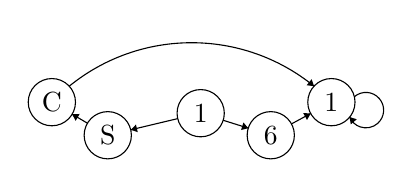
\begin{tikzpicture}[scale=0.1]
    \tikzstyle{every node}+=[inner sep=0pt]
    \draw [black] (26.7,-13.3) circle (3);
    \draw (26.7,-13.3) node {C};
    \draw [black] (45.6,-14.7) circle (3);
    \draw (45.6,-14.7) node {$1$};
    \draw [black] (33.8,-17.5) circle (3);
    \draw (33.8,-17.5) node {S};
    \draw [black] (54.5,-17.5) circle (3);
    \draw (54.5,-17.5) node {$6$};
    \draw [black] (62.2,-13.3) circle (3);
    \draw (62.2,-13.3) node {$1$};
    \draw [black] (42.68,-15.39) -- (36.72,-16.81);
    \fill [black] (36.72,-16.81) -- (37.61,-17.11) -- (37.38,-16.14);
    \draw [black] (31.22,-15.97) -- (29.28,-14.83);
    \fill [black] (29.28,-14.83) -- (29.72,-15.67) -- (30.23,-14.8);
    \draw [black] (48.46,-15.6) -- (51.64,-16.6);
    \fill [black] (51.64,-16.6) -- (51.03,-15.88) -- (50.73,-16.84);
    \draw [black] (57.13,-16.06) -- (59.57,-14.74);
    \fill [black] (59.57,-14.74) -- (58.62,-14.68) -- (59.1,-15.56);
    \draw [black] (28.907,-11.271) arc (129.11449:50.88551:24.638);
    \fill [black] (59.99,-11.27) -- (59.69,-10.38) -- (59.06,-11.15);
    \draw [black] (65.108,-12.614) arc (131.00538:-156.99462:2.25);
    \fill [black] (64.51,-15.19) -- (64.66,-16.12) -- (65.42,-15.47);
  \end{tikzpicture}
\end{center}
\rule{\linewidth}{0.4pt}

\begin{enumerate}
  \item \textbf{(4 pt.)} For each of the unlabeled binary trees, state whether
    or not it can be the structure of a red-black tree. If so, color the
    vertices red or black. If not, state which of the red-black tree invariants
    (1 to 5) cannot be satisfied and provide an explanation.

    \textbf{[We are expecting: A YES/NO, and either (1) a valid coloring or (2)
    a set of violated invariants and a brief explanation. For the colorings,
    feel free to redraw the trees by hand and upload the image.]}
    \begin{multicols}{2}
      \begin{enumerate}
        \item (1 point)

          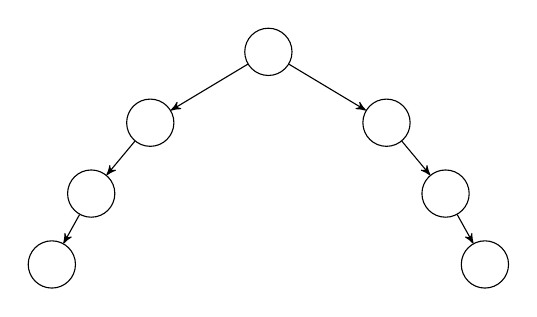
\begin{tikzpicture}[->,>=stealth',level/.style={sibling distance = 5cm/#1,level distance = 1.5cm},scale=0.6, transform shape]
            \node [treenode] {}
            child{
              node [treenode] {} 
              child{
                node [treenode] {} 
                child{
                  node [treenode] {} 
                }
                child[missing]
              }
              child[missing]
            }
            child{
              node [treenode] {}
              child[missing]
              child{
                node [treenode] {} 
                child[missing]
                child{
                  node [treenode] {} 
                }
              }
            };
          \end{tikzpicture}

        \item (1 point)

          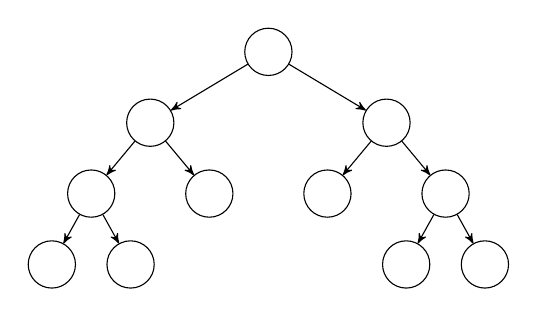
\begin{tikzpicture}[->,>=stealth',level/.style={sibling distance = 5cm/#1,level distance = 1.5cm},scale=0.6, transform shape]
            \node [treenode] {}
            child{
              node [treenode] {} 
              child{
                node [treenode] {} 
                child{
                  node [treenode] {} 
                }
                child{
                  node [treenode] {}
                }
              }
              child{
                node [treenode] {}
              }
            }
            child{
              node [treenode] {}
              child{
                node [treenode] {}
              }
              child{
                node [treenode] {}
                child{
                  node [treenode] {}
                }
                child{
                  node [treenode] {}
                }
              }
            };
          \end{tikzpicture}

        \item (1 point)

          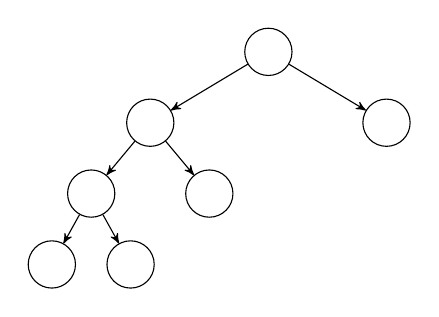
\begin{tikzpicture}[->,>=stealth',level/.style={sibling distance = 5cm/#1,level distance = 1.5cm},scale=0.6, transform shape]
            \node [treenode] {}
            child{
              node [treenode] {} 
                child{
                  node [treenode] {} 
                  child{
                    node [treenode] {} 
                  }
                  child{
                    node [treenode] {} 
                  }
                }
                child{
                  node [treenode] {} 
                }
            }
            child{
              node [treenode] {} 
            };
          \end{tikzpicture}

        \item (1 point)

          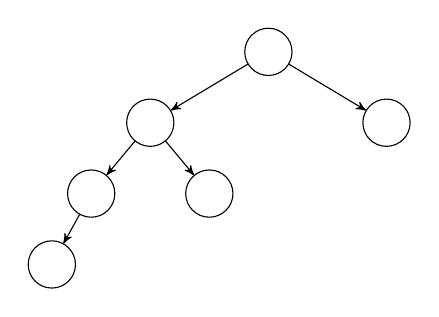
\begin{tikzpicture}[->,>=stealth',level/.style={sibling distance = 5cm/#1,level distance = 1.5cm},scale=0.6, transform shape]
            \node [treenode] {}
            child{
              node [treenode] {} 
                child{
                  node [treenode] {} 
                  child{
                    node [treenode] {} 
                  }
                  child[missing]
                }
                child{
                  node [treenode] {} 
                }
            }
            child{
              node [treenode] {} 
            };
          \end{tikzpicture}


      \end{enumerate}
    \end{multicols}

  \newpage

  \item \textbf{(4 pt.)} Give one example of a directed graph on four vertices,
    $A$, $B$, $C$, and $D$, such that both depth-first search and breadth-first
    search discover the vertices in the same order when started at A. Give one
    example of a directed graph where DFS and BFS discover the vertices in a
    different order when started at $A$. ``Discover'' means the time that the
    algorithm first reaches the vertex, referred to as \texttt{start\_time}
    during lecture. Assume that both DFS and BFS iterate over outgoing
    neighbors in alphabetical order.

    \textbf{[We are expecting a drawing of your graphs and an ordered list of
    vertices discovered by DFS and BFS.]}
\end{enumerate}

\newpage

\section*{Problems}

You can collaborate with your classmates about the problems. However:

\begin{itemize}
  \item Try the problems on your own \textit{before} collaborating.
  \item Write up your solutions yourself, in your own words.  You should never
    share your typed-up solutions with your collaborators.
  \item If you collaborated, list the names of the students you collaborated
    with at the beginning of each problem.
\end{itemize}

\noindent\rule{\linewidth}{1.0pt}

\begin{enumerate}

  \item \textbf{(Another topological sort algorithm)} \textbf{(7 pt.)} Consider
    a \textbf{complete directed acyclic graph} $G = (V, E)$ where $|V| = n$ and
    $|E| = \frac{n(n-1)}{2}$. Since the graph is complete, there exists an edge
    between each pair of the vertices $u, v \in V$ such that either
    $(u, v) \in E$ or $(v, u) \in E$ but not both (since the graph is acyclic).

    Suppose we define a function \texttt{contains(u,v)} which returns true if
    $(u, v) \in E$ and false if $(v, u) \in E$. Assume that we do not have
    access to the list of edges and can only access the graph through the
    \texttt{contains} function. (We do have access to the list of vertices
    though.)

    \begin{enumerate}
      \item (1 pt.) Give an asymptotically tight lower bound on the worst-case
      number of calls to \texttt{contains} required to find a topological sort
      of $G$.
      
      \textbf{[We are expecting: An asymptotic tight lower bound like 
      $\Omega(\ldots)$.]}

      \item (3 pt.) Prove that the bound is tight, i.e., that no algorithm can
      find a topological sort of $G$ with fewer than that many calls to
      \texttt{contains} in the worst-case.

      \textbf{[We expecting: A convincing argument.]}

      \item (3 pt.) Describe an algorithm that achieves this bound.

      \textbf{[We are expecting: Either an English description or pseudocode 
      of the algorithm, and an English justification of why it achives the
      bound.]}
    \end{enumerate}

  \item \textbf{(Gossip modeling}) \textbf{(9 pt.)} Suppose we have a community
    of $n$ people. We can create a directed graph from this community as
    follows: the vertices are people, and there is a directed edge from person
    $A$ to person $B$ if $A$ would forward a rumor to $B$. Assume that if there
    is an edge from $A$ to $B$, then $A$ will always forward any rumor they
    hear to $B$. Notice that this relationship isn't symmetric: $A$ might
    gossip to $B$ but not vice versa. Suppose there are $m$ directed edges
    total, so $G = (V,E)$ is a graph with $n$ vertices and $m$ edges.

    Define a person $P$ to be \em influential \em if for all other people $A$
    in the community, there is a directed path from $P$ to $A$ in $G$. Thus, if
    you tell a rumor to an influential person $P$, eventually the rumor will
    reach everybody. You have a rumor that you'd like to spread, but you don't
    have time to tell more than one person, so you'd like to find an
    influential person to tell the rumor to.
  
    In the following questions, assume that $G$ is the directed graph
    representing the community, and that you have access to $G$ as an array of
    adjacency lists: for each vertex $v$, in $O(1)$ time you can get a pointer
    to the head of the linked lists $v$\texttt{.outgoing\_neighbors} and
    $v$\texttt{.incoming\_neighbors}.  Notice that $G$ is not necessarily
    acyclic. In your answers, you may appeal to any statements we have seen in
    class, in the notes, or in CLRS.
  
    \begin{enumerate}
      \item (1 pt.) Show that all influential people in $G$ are in the same
        strongly connected component, and that everyone in this strongly
        connected component is influential.
      
      \textbf{[We are expecting: A short but formal proof.]}

      \item (5 pt.) Suppose that an influential person exists. Give an
        algorithm that, given $G$, finds an influential person in
        $O(n+m)$-time.

        \textbf{[We are expecting: Either an English description or pseudocode 
          of the algorithm, a formal proof of correctness, and an English
          justification of why it takes $O(n+m)$-time.]}

      \item (3 pt.) Suppose that you don't know whether or not an influential
        person exists. Use your algorithm from part (b) to give an algorithm
        that, given $G$, either finds an influential person in time $O(n+m)$
        if there is one, or else returns ``no influential person.''

        \textbf{[We are expecting: Either an English description or pseudocode 
          of the algorithm.]}
    \end{enumerate}
\end{enumerate}

\end{document}